\chapter{A Three-Stage DCF Framework for Mining Valuation}
\chapterstatus{Expanded reconstruction from Team 5. The original article
provides accounting reclassification, FCFF/FCFE, WACC, three-stage transition
and a reproducible synthetic Monte Carlo illustration. This chapter retains
those supported methods, corrects the terminal-value cash-flow definition and
adapts the framework to a finite-resource miner. Synthetic values are never
reported as Barrick estimates.}

\section{Valuation object: firm value before equity value}

% Sources: Team 5 ch-2, ch-4 and 3df; CONTENT-LEDGER BG-U-11.
Discounted cash flow is not one formula but a consistency system linking a
cash-flow definition, the claim being valued and the corresponding discount
rate. Team 5 distinguishes two coherent routes. The equity route discounts
free cash flow to equity at the cost of equity,
\begin{equation}
EqV_0=\sum_{y=1}^{H}\frac{FCFE_y}{\prod_{s=1}^{y}(1+k_{e,s})}
      +\frac{TV_H^{Eq}}{\prod_{s=1}^{H}(1+k_{e,s})},
\end{equation}
whereas the firm route discounts FCFF at WACC and values all operating claims
before financing:
\begin{equation}
EV_0=\sum_{y=1}^{H}\frac{FCFF_y}{\prod_{s=1}^{y}(1+w_s)}
     +\frac{TV_H^{Firm}}{\prod_{s=1}^{H}(1+w_s)}.
\end{equation}
The unified experiment adopts the firm route because the Team 4 operating
layer produces pre-financing drivers. For scenario \(m\), enterprise value is
converted to equity and then to a per-share quantity only through an explicit
bridge:
\begin{align}
EqV^{(m)}
  &=EV^{(m)}-\text{net debt}-\text{minority and other claims}
    +\text{admitted non-operating assets},\\
V_{ps}^{(m)}&=\frac{EqV^{(m)}}{N_{dil}}.
\end{align}
The signs, scale, currency, security and date of every bridge item are part of
the valuation result. A direct FCFE calculation cannot be used to hide an
unreconciled capital structure.

\begin{table}[H]
\centering
\small
\begin{tabularx}{\textwidth}{@{}p{2.7cm}p{3.0cm}p{2.8cm}X@{}}
\toprule
Route & Cash flow & Discount rate & Output and principal consistency test \\
\midrule
Firm valuation & FCFF before debt service & WACC & Enterprise value; operating
cash flows must exclude financing and be reconciled to invested capital. \\
Equity valuation & FCFE after net borrowing & Cost of equity & Equity value;
leverage policy and net borrowing must be modelled explicitly. \\
\bottomrule
\end{tabularx}
\caption{The two DCF routes recovered from Team 5. Mixing FCFF with the cost of
equity, or FCFE with WACC, changes the claim being valued and is inadmissible.}
\label{tab:dcf-route-consistency}
\end{table}

\section{Reclassifying financial statements for valuation}

% Sources: Team 5 ch-3; GAP-DCF-01 and GAP-VAL-05.
Standard statements mix operating, non-operating and financing items. Team 5's
reclassification is therefore a prerequisite, not an optional presentation
step. The operating side of invested capital can be expressed as
\begin{equation}
IC_y=OWC_y+PP\&E_y+\text{other net operating assets}_y,
\end{equation}
after excluding excess cash, marketable securities and other admitted
non-operating assets. The financing side must reconcile to debt and equity
claims. Return on invested capital is then
\begin{equation}
ROIC_y=\frac{NOPAT_y}{IC_{y-1}},
\end{equation}
so the comparison \(ROIC_y-w_y\) measures value creation from operating
capital rather than accounting earnings alone.

Operating working capital excludes cash and debt items that belong to the
financing bridge. In a mining application, inventories, receivables, payables,
royalties, reclamation provisions, streaming obligations and tax balances
must be assigned consistently. PP\&E and mine development also require care:
depreciation is an accounting allocation, sustaining capex is a cash outflow,
and closure liabilities are neither interchangeable nor automatically
contained in AISC.

NOPAT isolates after-tax operating profit from financing:
\begin{equation}
NOPAT_y=EBIT_y-\text{operating cash taxes}_y
       \approx EBIT_y(1-\tau_y),
\end{equation}
where the approximation is valid only when the tax rate and deferred-tax
adjustments are appropriate to the operating perimeter. Interest expense,
interest tax shields and income on excluded assets do not belong in NOPAT.

\begin{table}[H]
\centering
\small
\renewcommand{\arraystretch}{1.10}
\begin{tabularx}{\textwidth}{@{}p{3.0cm}p{4.2cm}X@{}}
\toprule
Block & Valuation treatment & Mining-specific control \\
\midrule
Revenue and operating cost & Build EBIT before financing. & Reconcile ounces,
realised price, ownership, royalties and whether cost metrics include D\&A or
sustaining investment. \\
Working capital & Include operating receivables, inventories and payables. &
Do not treat cash, debt or financing balances as operating working capital. \\
PP\&E and development & Link depreciation, capex and asset base. & Separate
sustaining, growth and closure expenditure; avoid counting AISC and capex
twice. \\
Taxes & Estimate operating cash taxes. & Separate current/deferred taxes,
jurisdictional effects and financing tax shields. \\
Non-operating and financing items & Exclude from FCFF and admit through the
EV-to-equity bridge. & Reconcile cash, debt, minorities, streams, other claims
and diluted shares to one filing date. \\
\bottomrule
\end{tabularx}
\caption{Financial-statement reclassification required before the operating
simulation can be called an FCFF model.}
\label{tab:dcf-reclassification}
\end{table}

\section{Operating forecasts and the FCFF contract}

% Sources: Team 5 ch-4 and ch-5; Team 4 interface.
Team 5 starts from sales, costs, margins, depreciation and working capital.
For a miner, the generic sales-growth shortcut is replaced by the more
informative component identity
\begin{equation}
Revenue_y^{(m)}=Q_y^{(m)}P_y^{realised,(m)}+\text{other operating revenue}_y^{(m)},
\end{equation}
where production \(Q\), realised price \(P^{realised}\), ownership and hedging
must share units and period conventions. Cost ratios can still be used as
checks, but a constant COGS-to-sales assumption is weak when grades, strip
ratios, energy, labour and mine mix change independently of price.

The admitted cash-flow identity is
\begin{align}
\text{Reinvestment}_y^{(m)}
  &=CapEx_y^{(m)}-D\&A_y^{(m)}+\Delta NWC_y^{(m)},\\
FCFF_y^{(m)}
  &=NOPAT_y^{(m)}-\text{Reinvestment}_y^{(m)}.
\end{align}
Every component uses the same sign convention: a rise in operating working
capital consumes cash, depreciation is non-cash, and capex consumes cash. CoS,
cash cost, AISC, royalties and D\&A cannot be combined until a data dictionary
proves what each aggregate already contains.

Team 5 also links growth to investment productivity. If expected operating
growth is \(g_y\) and the return on new invested capital is represented by
\(ROIC_y\), then
\begin{equation}
\text{reinvestment rate}_y=\frac{g_y}{ROIC_y},
\qquad
FCFF_y=NOPAT_y\left(1-\frac{g_y}{ROIC_y}\right).
\end{equation}
This identity prevents a model from assuming growth without funding it. It is
a consistency check rather than a licence to estimate Barrick's growth or
ROIC from the gold or equity-price series.

\section{Discount rate: currency, risk and capital structure}

% Sources: Team 5 ch-6; GAP-VAL-03/08.
Under the firm route, the pathwise or dated WACC is
\begin{equation}
w_y=\frac{E_y}{D_y+E_y}k_{e,y}
  +\frac{D_y}{D_y+E_y}k_{d,y}(1-\tau_y).
\end{equation}
A conventional CAPM estimate writes
\begin{equation}
k_{e,y}=R_{f,y}+\beta_y ERP_y+CRP_y,
\end{equation}
where any country-risk premium must match the geographic exposure and must not
be counted again in cash-flow haircuts. Beta requires an explicit convention:
a raw historical regression, smoothed beta or bottom-up unlevered/relevered
peer beta can produce different answers. The cost of debt may come from a
traded yield, recent borrowing spread or synthetic rating, but it must reflect
the same currency and horizon as the cash flows.

The risk-free input is conceptually a default-free zero-coupon rate matched to
the cash-flow maturity. A single long bond is only a proxy. Capital weights
should use market values and a target structure coherent with the forecast,
not book weights selected for convenience. If option-implied risk is already
embedded in the scenario distribution, the measure policy must also explain
why discounting does not charge for the same risk twice.

\section{Three stages and gradual convergence}

% Sources: Team 5 3df and montecarlo_int.
The three-stage model separates a high-growth or explicit phase, a transition
phase and a stable or closing phase. Its central contribution is gradual joint
convergence. Growth, operating margin, reinvestment, ROIC, leverage and risk
cannot jump independently at the terminal date. For a driver \(x\) that moves
from \(x_{hg}\) at the end of the first phase to \(x_s\) at year \(H\), a
transparent linear transition is
\begin{equation}
x_y=x_{hg}-\frac{y-H_1}{H-H_1}(x_{hg}-x_s),
\qquad H_1<y\leq H.
\end{equation}
The same device may be applied to several drivers, but their joint path must
remain economically coherent: lower growth normally implies lower incremental
reinvestment; mature margins and ROIC must be supportable; beta, leverage and
WACC should converge toward a defensible long-run state.

When perpetual continuation is economically admissible, Team 5's terminal
block is corrected to use post-horizon free cash flow rather than EBIT alone:
\begin{equation}
TV_H^{(m)}=
\frac{NOPAT_{H+1}^{(m)}
\left(1-g_s^{(m)}/ROIC_s^{(m)}\right)}
{w_H^{(m)}-g_s^{(m)}},
\qquad w_H^{(m)}>g_s^{(m)}.
\end{equation}
The denominator condition is necessary but not sufficient. Stable growth must
remain compatible with the valuation currency, long-run economy, reinvestment
capacity and return on new capital.

\section{Executable assumption register for the current experiment}
\label{sec:executable-valuation-assumptions}

The equations above describe the reusable method; this section discloses the
numbers actually passed to the current unified run. They are read from
\path{config/provisional_valuation_20260827_team4_separated.json}, not inferred
from the plotted valuation output. All four price branches use the same values.
They are deliberately classified as methodological assumptions because no
filing-level WACC, invested-capital reconstruction or mine-closure calibration
currently supports them as Barrick point estimates.

\begin{table}[H]
\centering
\caption{Editable non-gold parameters used by the current executable valuation.}
\label{tab:current-editable-valuation-parameters}
\scriptsize
\setlength{\tabcolsep}{3pt}
\renewcommand{\arraystretch}{1.10}
\begin{tabularx}{\textwidth}{@{}p{3.15cm}p{1.35cm}X X@{}}
\toprule
Configuration field & Current & Where it enters & Interpretation and effect \\
\midrule
\texttt{model.tax\_rate} & 25.0\% & Converts component margin to an
after-tax proxy. & Higher tax lowers explicit and terminal FCFF. \\
\texttt{model.high\_growth} & 8.5\% & First point of the five-year linear
growth schedule. & Raises early reinvestment through \(g/ROIC\); it does not
directly grow the operating margin paths. \\
\texttt{model.stable\_growth} & 2.5\% & Last schedule point and terminal
growth \(g_s\). & Changes terminal reinvestment and the \(w-g\) denominator. \\
\texttt{model.roic\_high} & 14.5\% & First point of the ROIC schedule. & At
fixed growth, higher ROIC reduces required reinvestment. \\
\texttt{model.roic\_stable} & 10.5\% & Last ROIC and terminal return. & Sets
terminal reinvestment \(g_s/ROIC_s=23.81\%\). \\
\texttt{model.wacc\_0} & 9.1\% & Initial state of the WACC process. & Affects
the conditional path from which years 1--5 are drawn. \\
\texttt{model.wacc\_long\_run} & 8.3\% & Mean-reversion level. & Pulls later
discount rates toward 8.3\%. \\
\texttt{model.wacc\_reversion} & 0.45 & Annual reversion speed. & Controls how
quickly the initial 9.1\% approaches the long-run level. \\
\texttt{model.wacc\_volatility} & 0.9\% & Diffusion scale of annual WACC. &
Widens the discount-rate and terminal-value distributions. \\
\texttt{model.terminal\_}\newline\texttt{spread\_floor} & 1.0\% & Lower-bound distance above
stable growth. & Enforces \(w_y\geq g_s+1\%=3.5\%\), with a separate 25\% cap. \\
\texttt{equity\_bridge.*} & zeros & EV-to-equity bridge. & Debt, cash,
minorities, other claims and non-operating assets are unresolved placeholders. \\
\texttt{diluted\_shares\_mn} & 1,675.51 & Equity value per share. & Unreconciled
proxy; changing it rescales every per-share distribution. \\
\bottomrule
\end{tabularx}
\end{table}

The five annual schedule points are generated by \texttt{numpy.linspace}.
Growth therefore moves through 8.5\%, 7.0\%, 5.5\%, 4.0\% and 2.5\%; ROIC moves
through 14.5\%, 13.5\%, 12.5\%, 11.5\% and 10.5\%. The corresponding
reinvestment rates are 58.62\%, 51.85\%, 44.00\%, 34.78\% and 23.81\%.
Figure~\ref{fig:current-dcf-driver-schedule} is generated by the valuation code
from those exact run inputs, and its CSV/JSON sidecars retain every plotted
number and field name.

\IfFileExists{img/valuation/dcf_driver_schedule.png}{%
  \begin{figure}[H]
    \centering
    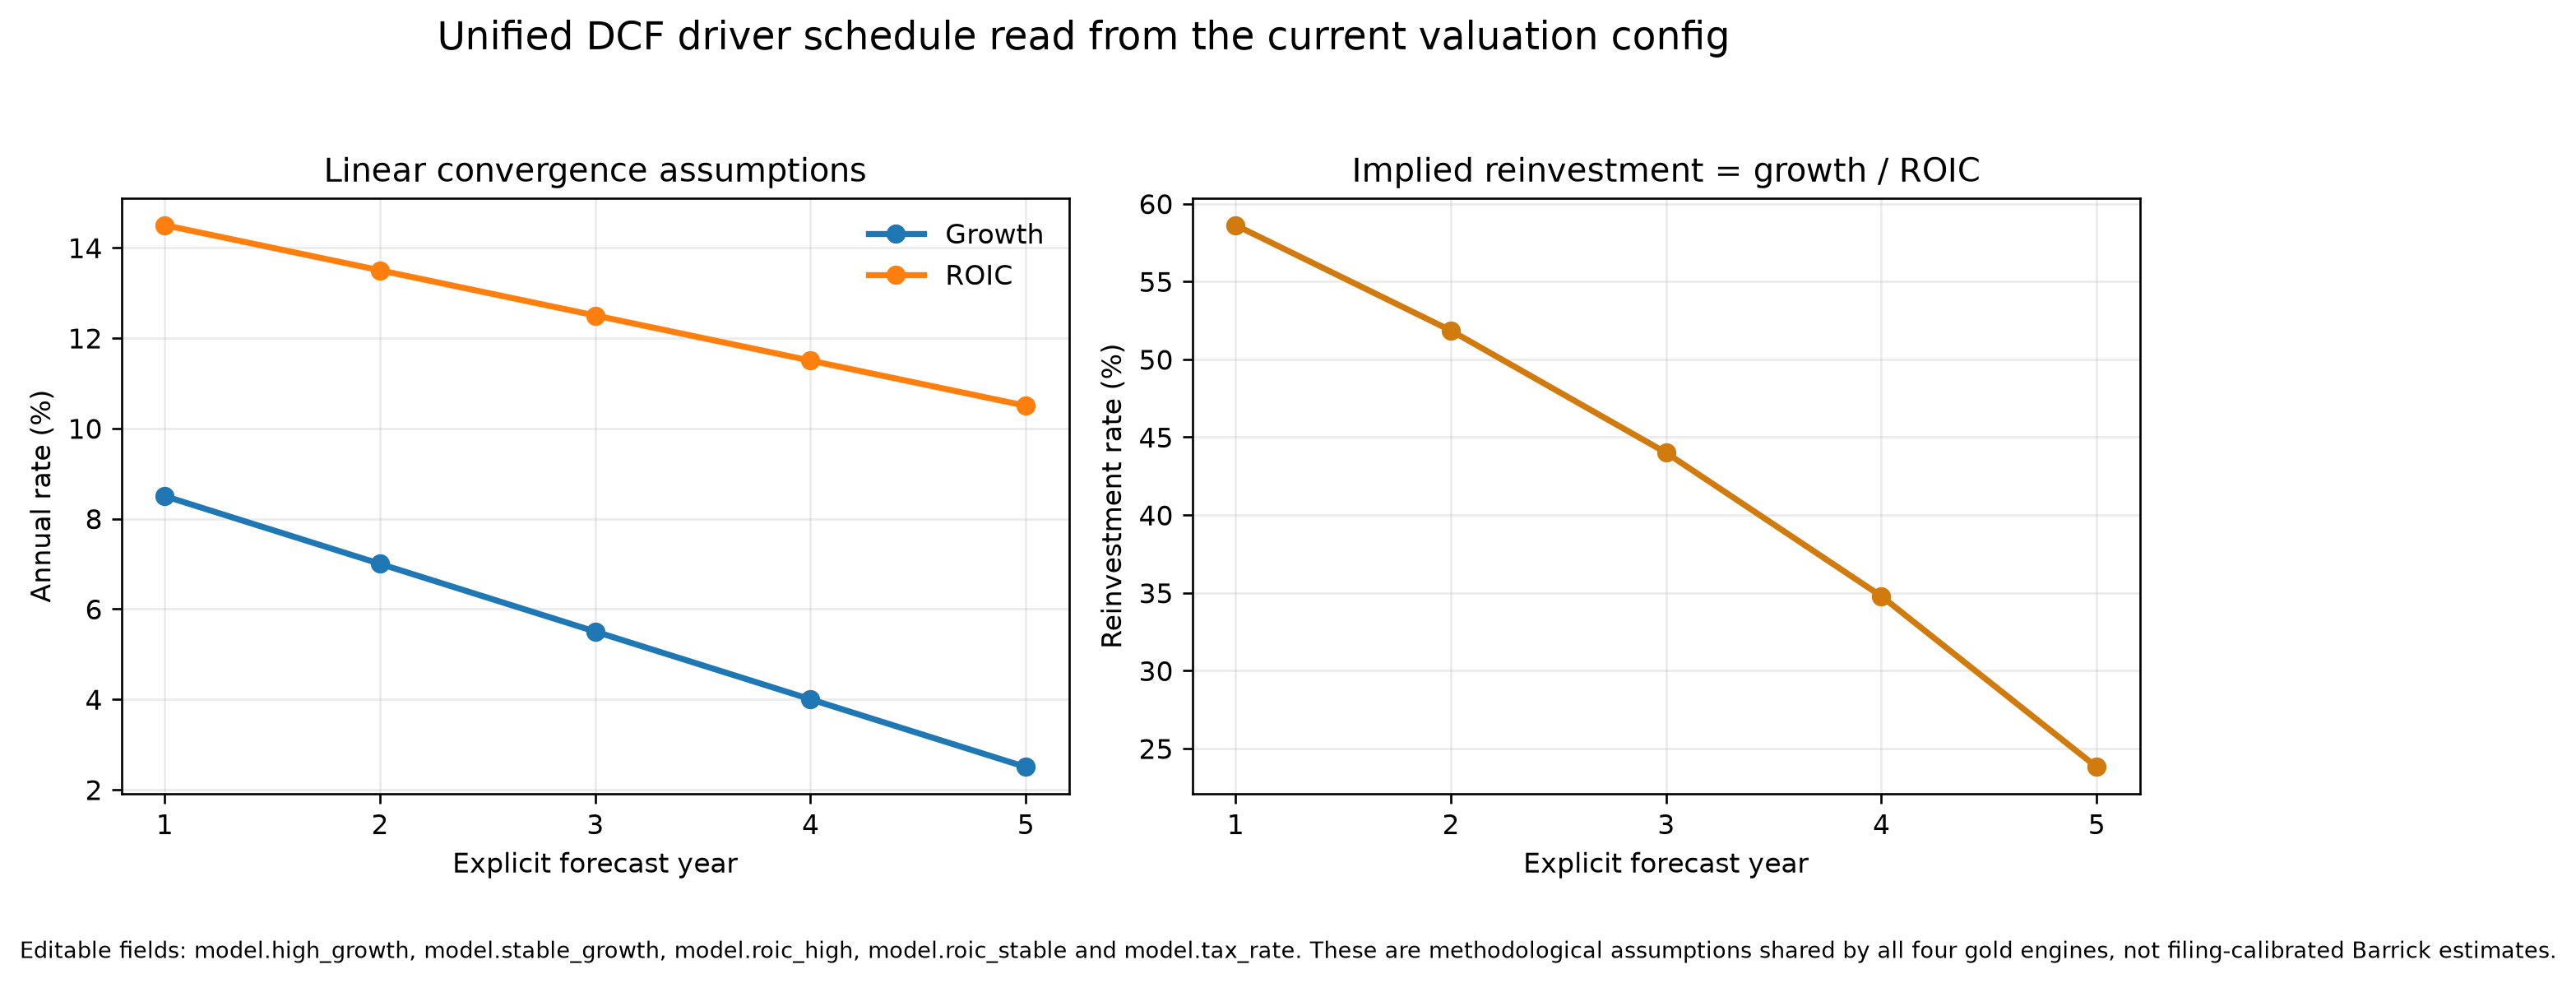
\includegraphics[width=0.98\textwidth]{img/valuation/dcf_driver_schedule.png}
    \caption{Growth, ROIC and implied reinvestment schedule used by the current
    run. These common DCF assumptions do not vary across the four gold-price
    engines.}
    \label{fig:current-dcf-driver-schedule}
  \end{figure}
}{%
  \gapbox{The generated DCF-driver dashboard is unavailable; no editorially
  reconstructed substitute is admitted.}%
}

The annual WACC is not a manually descending list. Starting from \(w_0=9.1\%\),
the code applies
\begin{align}
w_{y+1}&=\bar w+(w_y-\bar w)e^{-\kappa}
       +\sigma_c\varepsilon_{y+1},\\
\sigma_c&=\sigma_w
\sqrt{\frac{1-e^{-2\kappa}}{2\kappa}},
\end{align}
with \(\bar w=8.3\%\), \(\kappa=0.45\), \(\sigma_w=0.9\%\) and independent
standard-normal shocks. The zero-shock path is approximately 8.81\%, 8.63\%,
8.51\%, 8.43\% and 8.38\% for years 1--5. The actual valuation uses 8,192
stochastic WACC paths, created once with seed 20260827 and reused byte-for-byte
under every gold model. Thus the shaded interval in
Figure~\ref{fig:current-wacc-assumption-paths} is discount-rate uncertainty,
whereas differences between model valuation distributions still isolate the
price engine.

\IfFileExists{img/valuation/wacc_assumption_paths.png}{%
  \begin{figure}[H]
    \centering
    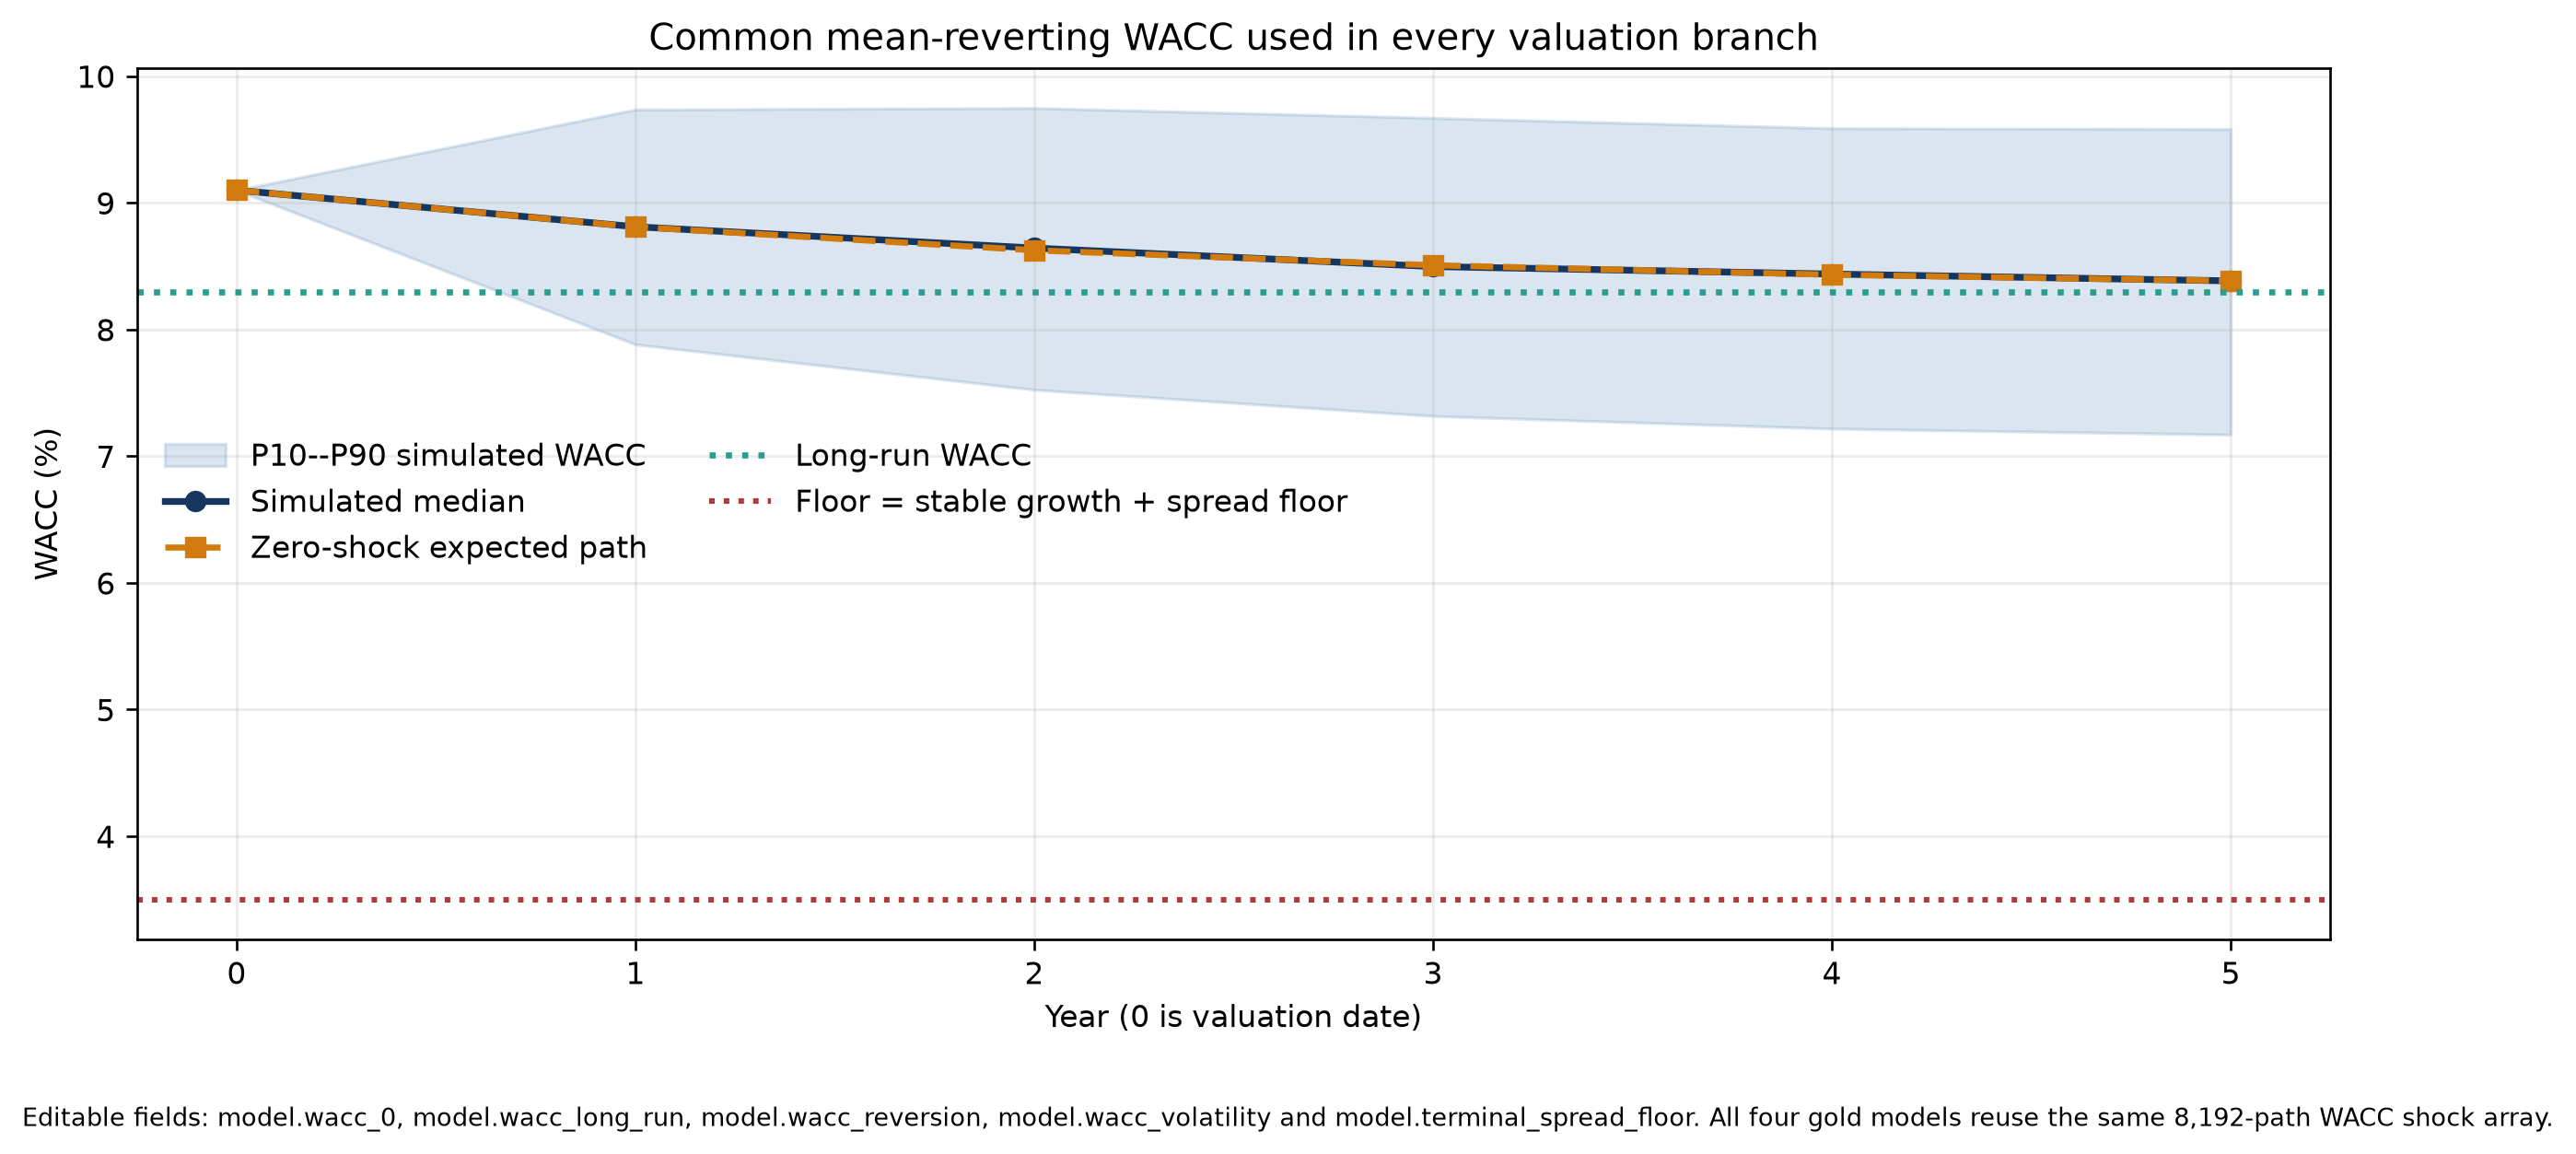
\includegraphics[width=0.95\textwidth]{img/valuation/wacc_assumption_paths.png}
    \caption{Initial WACC, zero-shock mean-reversion path, simulated
    P10--P90 envelope, 8.3\% long-run level and terminal-spread floor used in
    the common valuation layer.}
    \label{fig:current-wacc-assumption-paths}
  \end{figure}
}{%
  \gapbox{The generated WACC-assumption dashboard is unavailable; no
  substitute path is supplied manually.}%
}

The terminal block applies the final positive after-tax component margin,
grows it once, funds stable growth at \(g_s/ROIC_s\), capitalises the resulting
FCFF at \(w_H-g_s\), and then discounts it back over the same path. The left
panel of Figure~\ref{fig:current-terminal-value-mechanics} makes the two most
sensitive editable inputs visible without pretending that the normalized
multiple is a company estimate. The right panel uses the accepted run and
reports how much of positive enterprise value comes from the discounted
terminal block under each price engine. This is the appropriate place to judge
whether the five-year horizon leaves excessive weight in the terminal value.

\IfFileExists{img/valuation/terminal_value_mechanics.png}{%
  \begin{figure}[H]
    \centering
    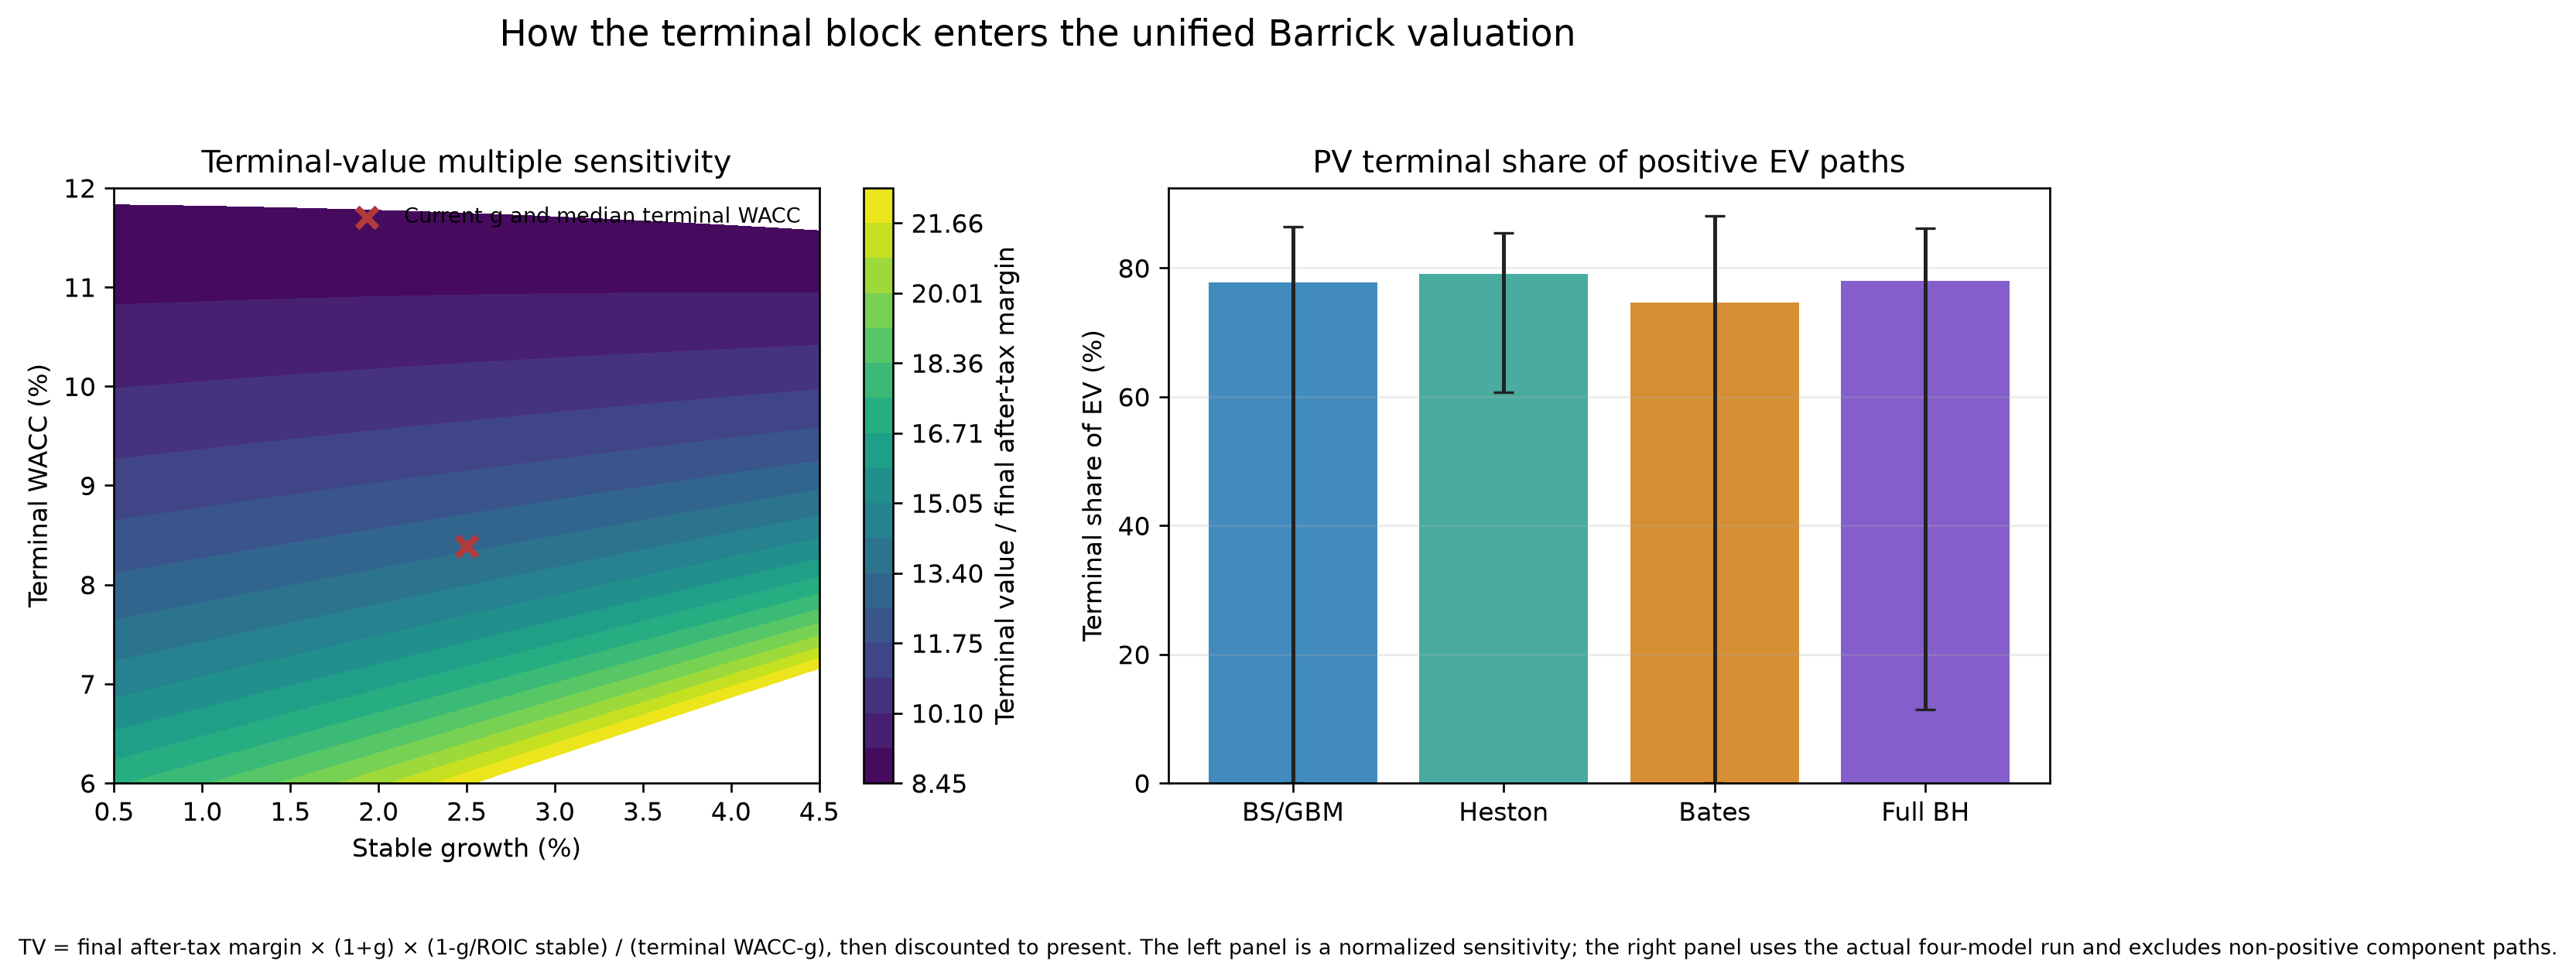
\includegraphics[width=0.99\textwidth]{img/valuation/terminal_value_mechanics.png}
    \caption{Terminal-value mechanics. Left: normalized sensitivity to stable
    growth and terminal WACC at the current stable ROIC. Right: actual-run
    P10, median and P90 terminal contribution to positive enterprise-value
    paths.}
    \label{fig:current-terminal-value-mechanics}
  \end{figure}
}{%
  \gapbox{The generated terminal-value dashboard is unavailable; no manually
  reconstructed sensitivity is admitted.}%
}

This register also clarifies how the project is joined. Team~8 changes only the
gold path; the Barrick/Team~4 operating vector is common; the tax,
growth--ROIC reinvestment rule, WACC array and terminal policy are common; and
the unresolved equity bridge is applied last. Consequently, editing any field
in Table~\ref{tab:current-editable-valuation-parameters} changes all four
branches together. Editing a Team~8 parameter changes only its corresponding
gold-price branch. No Team~4 simulated gold price or demonstrator valuation is
used.

\section{Finite-resource closure for a mining company}

Perpetual growth is not the automatic base case for a miner because reserves,
mine lives and closure obligations are finite. The terminal policy must connect
the explicit asset horizon to depletion, replacement, exploration and future
portfolio renewal. The alternatives in Table~\ref{tab:terminal-closure-alternatives}
are mutually exclusive modelling choices rather than terms to be blended.

\begin{table}[H]
\centering
\caption{Terminal-closure alternatives that must be chosen, not blended.}
\label{tab:terminal-closure-alternatives}
\small
\renewcommand{\arraystretch}{1.12}
\begin{tabularx}{\textwidth}{@{}p{3.00cm}X X@{}}
\toprule
Closure & Required evidence & Main risk \\
\midrule
Finite asset run-off & Mine lives, production decline, closure liabilities and
post-closure cash flows. & Omitting unmodelled replacement or corporate costs. \\
Explicit portfolio renewal & Exploration, development and acquisition
reinvestment tied to additions and future production. & Treating speculative
replacement as certain or costless. \\
Corporate going concern & Sustainable post-horizon FCFF, growth, ROIC, WACC
and continuing asset policy. & Hiding finite-resource economics inside a
perpetual-growth denominator. \\
\bottomrule
\end{tabularx}
\end{table}

\section{From deterministic DCF to a stochastic valuation distribution}

% Sources: Team 5 montecarlo_int, simulation_results and scenarios.
Team 5 extends the three-stage model without changing its accounting logic.
For each draw \(m\), it generates joint paths for operating drivers and WACC,
constructs FCFF, applies pathwise discount factors
\begin{equation}
DF_y^{(m)}=\prod_{s=1}^{y}\frac{1}{1+w_s^{(m)}},
\end{equation}
and returns
\begin{equation}
EV^{(m)}=\sum_{y=1}^{H}FCFF_y^{(m)}DF_y^{(m)}
       +TV_H^{(m)}DF_H^{(m)}.
\end{equation}
The reporting object is the empirical distribution
\(\{EV^{(1)},\ldots,EV^{(M)}\}\), summarised by its median, tail quantiles,
dispersion, terminal-value share and sensitivity measures. Dependence is part
of the model: weak operating states may coincide with higher discount rates,
and growth, margins, ROIC and reinvestment must move as a coherent narrative.

The accepted Team~5 contribution is methodological: distributions, fan
charts, terminal-value shares and driver attribution must be reported, and
Monte Carlo sampling error must be separated from economic dispersion. Its
standalone numerical example uses synthetic value units and is therefore
retained only as a branch-level implementation test. It is intentionally not
shown as Barrick evidence and contributes no simulated company price to the
unified valuation.

The scenario extension similarly varies coherent assumption sets rather than
one cell at a time. In the source illustration, conservative, base and
expansion cases jointly change growth, margin, ROIC, WACC and volatility. The
numerical values remain synthetic, but three methodological controls carry
into the thesis: every scenario must state its joint economic narrative; a
wider absolute distribution can accompany a stronger scenario; and the
terminal-value share must be reported because it can rise as stable economics
improve.

\section{Barrick-specific implementation contract}

The original Team 5 engine is a reproducible synthetic benchmark. It becomes
a Barrick valuation only after every illustrative driver is replaced by a
dated, unit-checked input and the finite-resource closure is selected. The
following table separates completed methodological reuse from open economic
reconciliation.

\begin{table}[H]
\centering
\caption{Team 5 contribution and Barrick-specific admission gate.}
\label{tab:dcf-reuse-gates}
\small
\renewcommand{\arraystretch}{1.12}
\begin{tabularx}{\textwidth}{@{}p{2.7cm}X X@{}}
\toprule
Element & Reusable contribution & Required before a validated Barrick claim \\
\midrule
Accounting perimeter & Operating/non-operating/financing reclassification,
NOPAT and invested-capital logic. & Filing-level mapping for Barrick, with
mining cost, D\&A, capex, tax and closure definitions reconciled. \\
FCFF engine & NOPAT, reinvestment and pathwise discounting identities. & Team
4-to-EBIT bridge, working capital, sustaining/growth capex and dimensional
tests. \\
WACC & Cost-of-equity/debt and capital-weight architecture. & Dated currency-
consistent risk-free curve, ERP, beta, borrowing spread, tax and market-value
weights. \\
Three-stage closure & Joint transition and growth--ROIC--reinvestment
consistency. & Mine horizon and one explicit, tested run-off, renewal or going-
concern policy. \\
Stochastic DCF & Distributional estimator, fan charts, quantiles, terminal
share and sensitivity reporting. & Approved joint scenarios, measure policy,
seeds, convergence and dependence diagnostics. \\
Equity bridge & Enterprise-versus-equity distinction. & Dated net debt, cash,
minorities, streams, other claims, non-operating assets and diluted shares. \\
\bottomrule
\end{tabularx}
\end{table}

The next chapter uses this architecture as a common contract across four gold-
price engines. It reports the conditional Barrick experiment and its validation
in one place; the calibration and predictive evidence itself remains in
Chapter~9 and is not repeated.
